% Numeric oracle: the edge pen must not enlarge the node's own outer contour.
\documentclass{article}
\usepackage{tikz}
\usetikzlibrary{arrows.meta,shapes.geometric}
\begin{document}
\makeatletter
\newcommand{\reportpath}[1]{\pgfgetpath\savedpath\typeout{SHAPE #1: \meaning\savedpath}}
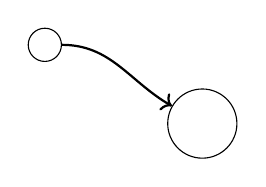
\begin{tikzpicture}
  \node[circle,draw,minimum size=12pt,inner sep=0pt] (source) at (-2,1) {};
  \node[circle,draw,minimum size=25pt,inner sep=0pt] (target) at (0,0) {};
  \draw[->,thick] (source) to[out=0,in=150] (target) \pgfextra{\reportpath{circle}};
\end{tikzpicture}
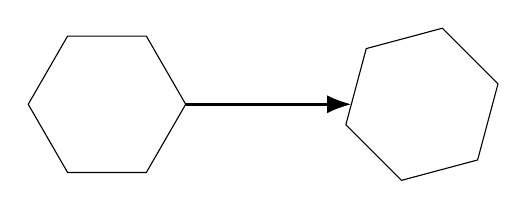
\begin{tikzpicture}
  \node[draw,regular polygon,regular polygon sides=6,minimum size=2cm,inner sep=0pt] (flat) at (0,0) {};
  \node[draw,regular polygon,regular polygon sides=6,regular polygon rotate=15,minimum size=2cm,inner sep=0pt] (rotated) at (4,0) {};
  \foreach \pen in {thin,very thick}{%
    \draw[-{Latex[length=3mm]},\pen] (flat) to[out=0,in=180] (rotated) \pgfextra{\reportpath{hexagon-\pen}};}
\end{tikzpicture}
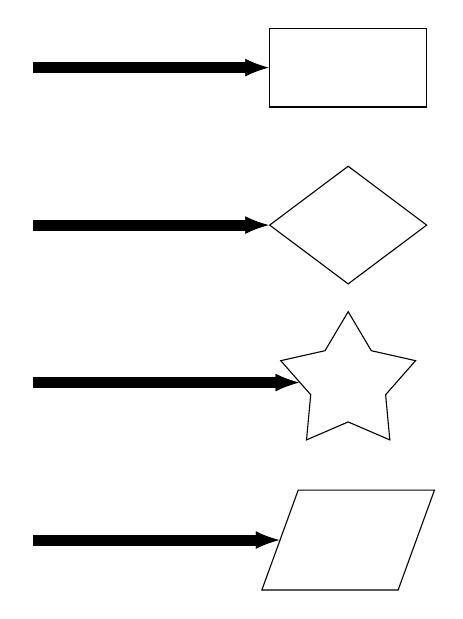
\begin{tikzpicture}
  \node[draw,rectangle,minimum width=2cm,minimum height=1cm,inner sep=0pt] (rect) at (0,3) {};
  \node[draw,diamond,aspect=1.4,minimum width=2cm,minimum height=1.5cm,inner sep=0pt] (diamond) at (0,1) {};
  \node[draw,star,star points=5,star point ratio=1.8,minimum size=1.8cm,inner sep=0pt] (star) at (0,-1) {};
  \node[draw,trapezium,trapezium left angle=70,trapezium right angle=110,minimum width=2.2cm,minimum height=1.2cm,inner sep=1pt] (trap) at (0,-3) {};
  \foreach \name/\y in {rect/3,diamond/1,star/-1,trap/-3}{%
    \draw[-{Latex[length=3mm]},thin] (-4,\y) to[out=0,in=180] (\name) \pgfextra{\reportpath{\name-thin}};
    \draw[-{Latex[length=3mm]},line width=4pt] (-4,\y) to[out=0,in=180] (\name) \pgfextra{\reportpath{\name-thick}};}
\end{tikzpicture}
\begin{tikzpicture}
  \node[draw,trapezium,trapezium left angle=70,trapezium right angle=110,minimum width=4cm,minimum height=2cm,inner sep=1pt] (trap) at (0,0) {};
  \foreach \anchor in {center,top right corner,29.608981225488687}{%
    \pgfpointanchor{trap}{\anchor}\typeout{TRAPEZIUM ANCHOR \anchor: \the\pgf@x,\the\pgf@y}}
  \draw[-{Latex[length=3mm]},thin] (6,6) to[out=180,in=29.608981225488687] (trap) \pgfextra{\reportpath{miter-thin}};
  \draw[-{Latex[length=3mm]},line width=6pt] (6,6) to[out=180,in=29.608981225488687] (trap) \pgfextra{\reportpath{miter-thick}};
\end{tikzpicture}
\makeatother
\end{document}
